\chapter{Implementation}


\section{Hierarchy of Arrays}

The API of an array is defined by an interface called INDArray which has a dense implementation for each backend: NDArray class for the CPU and JCublasNDArray class for the GPU. But since most of the operations and methods are shared between the two backends, they are implemented in an abstract class called BaseNDArray.

Adding sparse representations asked two questions:
\begin{enumerate}
 	\item What can be shared with the dense arrays ?
	\item What can be between the different sparse arrays and what are format-specific ?
\end{enumerate}

To answer those questions, we need to go a little bit deeper in the implementation. 

The dense implementation includes methods that are inherently related to the way dense ndarray is internally made, and other methods are related to the generic parameters such as the shape or are utility method.

The first type of methods is not useful in case of sparse. Dense and sparse ndarrays aren't built in the same manner. Methods such as \textit{getStrides} aren't relevant in the sparse context. Reciprocally the sparse array will need methods which will be irrelevant in the dense context.

We encounter the same situation between the different sparse formats. Some will need utily methods that the other ones won't need.

But everything has to be defined in the INDArray interface. To avoid code duplication, everything than can be shared should be implemented in the higher level of the hierarchy. The methods that are not compatible with a type of ndarray will simply throw an unsupported operation exception.

The drawback brought with this solution is that we always need to verify the type of the ndarray before doing any operations.

// TODO update schema
 
\begin{figure}[H]
	\begin{center}
		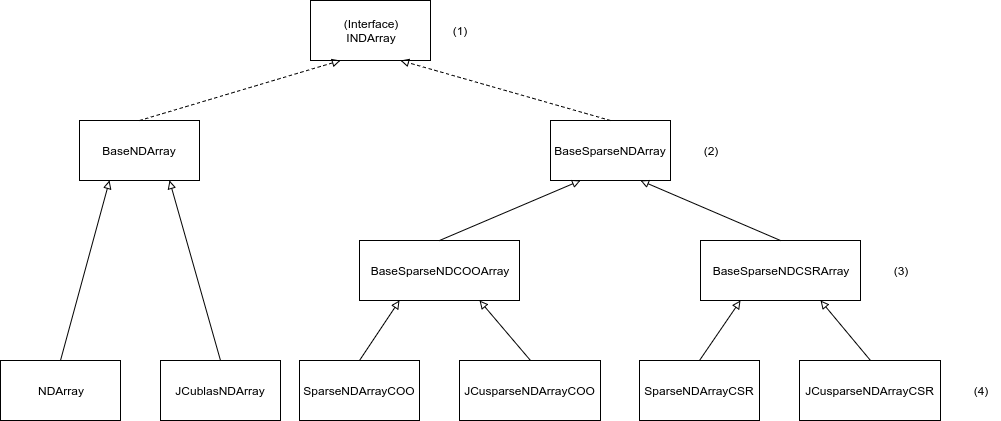
\includegraphics[width=6.5in]{images/INDArrayHierarchy.png} 
		\label{fig:hierarchy}
		\caption{Arrays hierarchy in Nd4j}
	\end{center}
\end{figure}


\section{Limitations and Constraints}

Nd4j has been made in the perspective of dense arrays. The design has been optimized rearding the dense implementation. 

\subsection{DataBuffers have a fixed length}
\subsection{Workspaces}

\section{CSR Matrices}
\subsection{Structure}
\subsection{Get or Put Data into this format}
\subsection{Limits with this format}

\section{COO Tensors}
\subsection{First implementation}

\subsection{More parameters are needed to define the tensors}
\subsubsection{All and Interval Indexes}
\subsubsection{Point Index}
\subsubsection{Specified Index}
\subsubsection{New Axis Index}

\subsection{Computations of the the Parameters}
\subsubsection{Computation of the Sparse Offsets}
\subsubsection{Computation of the Flags}
\subsubsection{Computation of the Hidden Dimensions}

\subsection{Sparse Indexes Translation}
..